\documentclass[11pt]{amsbook}

\usepackage{../HBSuerDemir}	% ------------------------

\begin{document}

% ++++++++++++++++++++++++++++++++++++++
\hPage{b2p1/121}
% ++++++++++++++++++++++++++++++++++++++

A bound (position) vector $\vec{r} = \vec{OP}$ having its initial point at the origin and extremity at $P(x, y, z)$ defines uniquely the point $P$ and conversely, and we make no difference between the symbols $\vec{OP}, \vec{P}, P, \vec{r}, (x, y, z)$ and write

\[
	\vec{r} = \vec{OP} = \vec{P} = P = (x, y, z)
\]
which is a \underline{coordinate vector}.
\begin{figure}[htb]
	\centering
	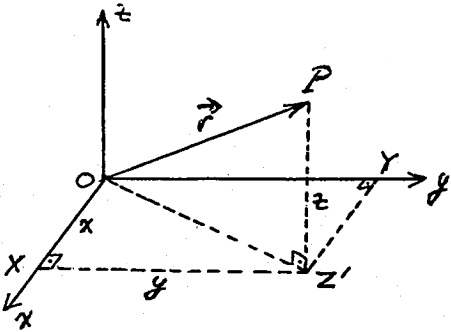
\includegraphics[width=0.5\textwidth]{images/b2p1-121-fig01}
\end{figure}
\\
Any free vector can be expressed as a coordinate vector.
\\
Since $(x, y, z)$ is an ordered triple, it can be considered as an element of the cartesian product $R \times R \times R = R^3$.
\\
We represent the position vector $(x, y, z)$ as the column matrix

\[
	\begin{bmatrix}
		x\\
		y\\
		z
	\end{bmatrix}
	=
	\begin{bmatrix}
		x, y, z
	\end{bmatrix}^{T}
\]
\subsubsection{Length of a vector}:
\label{subsubsec:Lengthofavector}
\\
Referring to above Figure we have as the length $|\vec{OP}|$ of the vector $\vec{OP}$:
\begin{align*}	
	|\vec{OP}|^2 = |OP|^2 &= |OZ'|^2 + |Z'P|^2
	\\
	&= (|x|^2 + |y|^2) + |z|^2 = x^2 + y^2 + z^2
	\\
	\implies
	|P| = |\vec{OP}| &= \sqrt{x^2 + y^2 + z^2} (\geq 0)
\end{align*}

\underline{Example.} Find the lenghts of
\[
	A = (1, -2, 2), B = (2, 3, 6), C = (\frac{1}{9}, \frac{4}{9}, \frac{8}{9})
\]
\underline{Solution.}
\begin{align*}	
	|A| &= \sqrt{1^2 + (-2)^2 + 2^2} = \sqrt{1 + 4 + 4} = 3
	\\
	|B| &= \sqrt{4 + 9 + 36} = 7
\end{align*}

% =======================================================
\end{document}  

%==== templates ====

%==== environments ====

%\begin{figure}[htb]
%	\centering
%	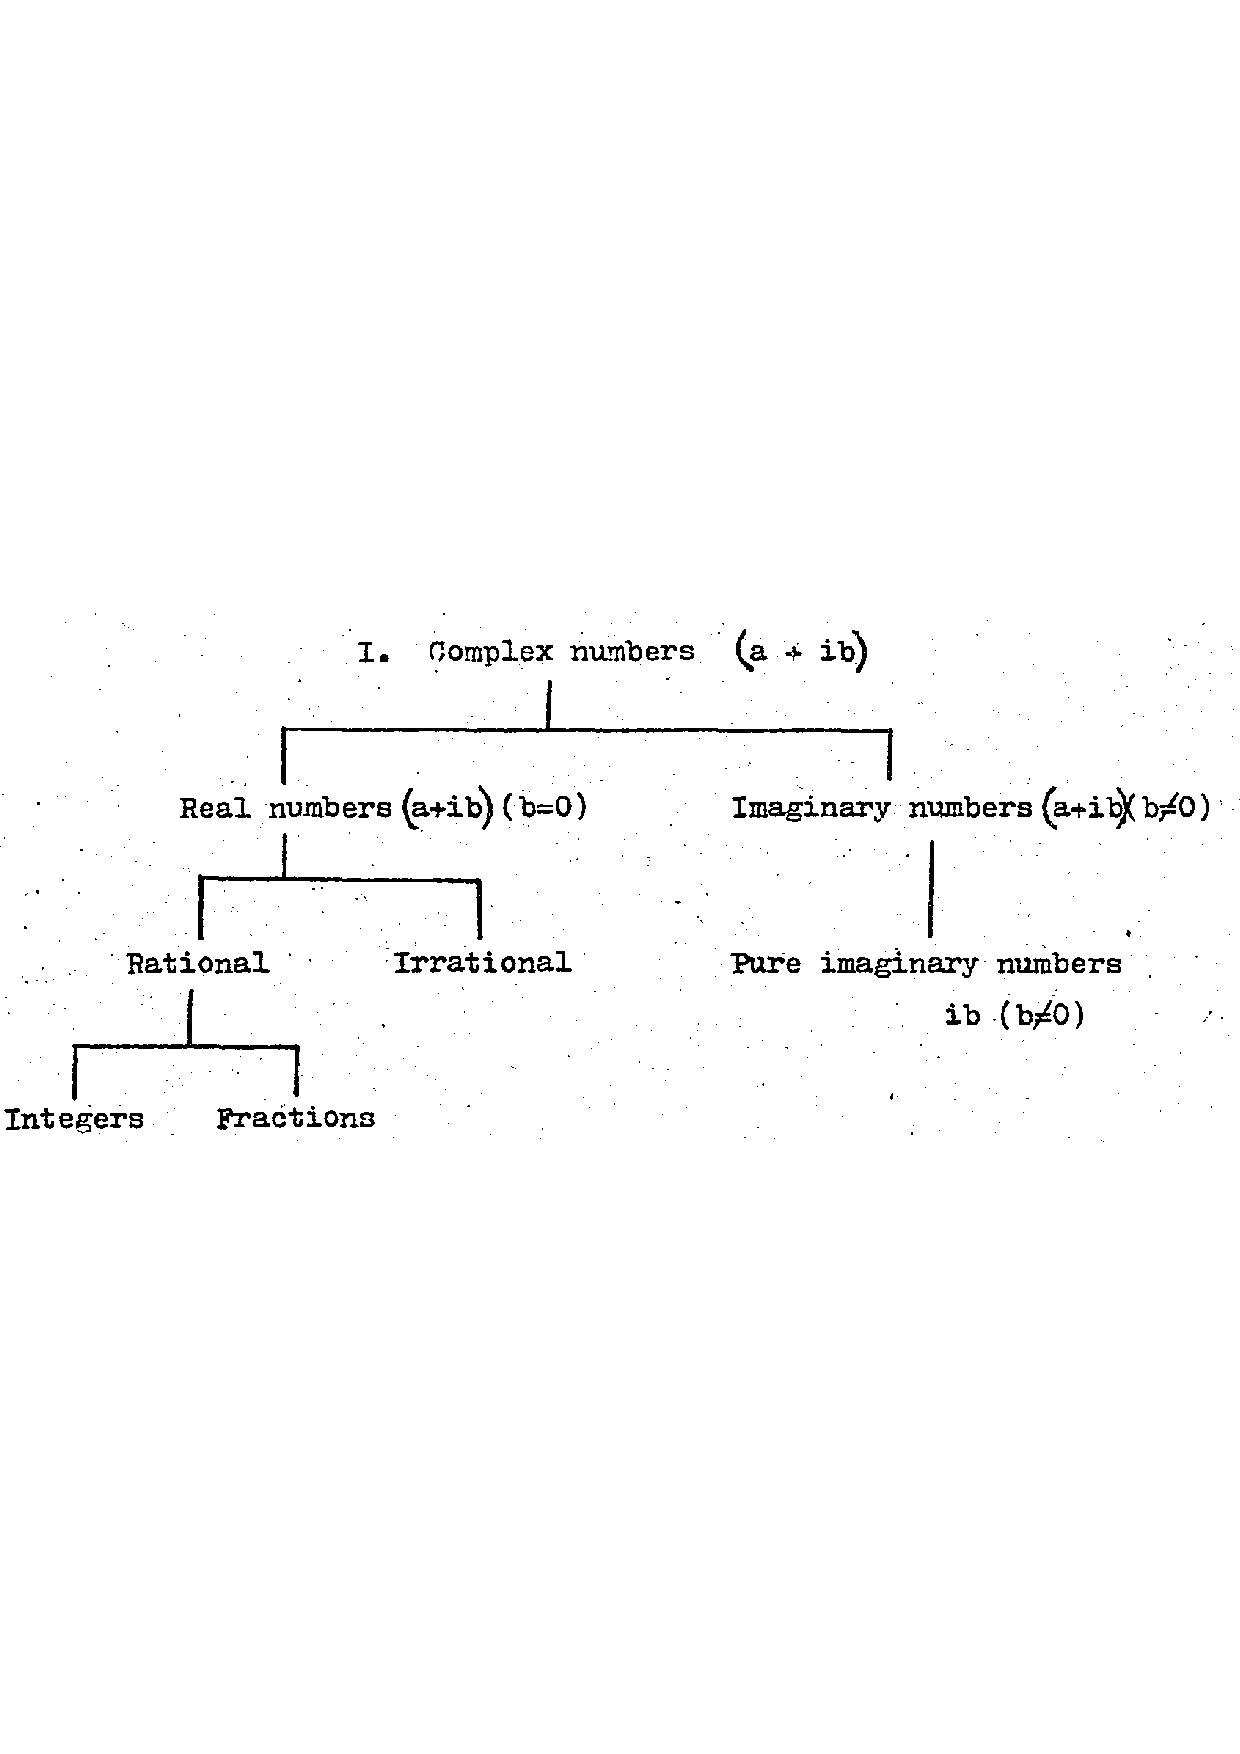
\includegraphics[width=0.9\textwidth]{images/SD-1-1p15A}
%	\caption{Classification of complex numbers}
%	\label{fig:classificationOfComplexNumbersA}
%\end{figure}

%\begin{center}
%\begin{tabular}{cc}
%\end{tabular}
%\end{center}

%\begin{exmp}
%\begin{hSolution}
%\end{hSolution}
%\end{exmp}

%\begin{hEnumerateAlpha}
%\end{hEnumerateAlpha}

%\begin{hEnumerateRoman}
%\end{hEnumerateRoman}

%$
%\begin{bmatrix}
%\end{bmatrix}
%$

%\frac{aaaa}{bbb}
%\frac{a_{n}}{b_{n}}
%\left( aaaa \right)
%\Longrightarrow

%\begin{multicols}{2}
%	bb
%\columnbreak
%	aa
%\end{multicols}
